\documentclass[aps,%
14pt,%
final,%
oneside,
onecolumn,%
musixtex, %
superscriptaddress,%
centertags]{extarticle} %% 
\usepackage[english,russian]{babel}
\usepackage[utf8]{inputenc}
%всякие настройки по желанию%
\usepackage[colorlinks=true,linkcolor=blue,unicode=true]{hyperref}
\usepackage{euscript}
\usepackage{supertabular}
\usepackage[pdftex]{graphicx}
\usepackage{amsthm,amssymb, amsmath}
\usepackage{textcomp}
\usepackage[bottom=20mm, top=20mm, left=30mm, right=15mm]{geometry}

\begin{document}

\begin{titlepage} 
\begin{center}
% Upper part of the page
{\large САНКТ-ПЕТЕРБУРГСКИЙ \\ ГОСУДАРСТВЕННЫЙ УНИВЕРСИТЕТ} \\[1.0cm]
{\large Математическое обеспечение и администрирование информационных систем} \\[0.2cm]
{\large Системное программирование} \\[3.5cm]
 
% Title
\textbf{\Large Назаренко Владимир Владимирович} \\[1cm]
\textbf{\LARGE Выделение объектов на видеопоследовательности}\\[1.0cm]
{\Large Выпускная квалификационная работа} \\[3.5cm]

%supervisor
\begin{flushright} \large
\emph{Научный руководитель:} \\
ст. преп. \textsc{Смирнов М. Н.}
\end{flushright}
 \begin{flushright} \large
\emph{Рецензент:} \\
\textsc{Пенкрат Н. А.} \\
менеджер проектов, ООО ``Ланит-Терком''
\end{flushright}
\vfill 

% Bottom of the page
{\large {Санкт-Петербург}} \par
{\large {2018 г.}}
\end{center} 
\end{titlepage}

\begin{titlepage} 
\begin{center}
% Upper part of the page
{\large SAINT PETERSBURG STATE UNIVERSITY} \\[1.0cm]
{\large Software and Administration of Information Systems} \\[0.2cm]
{\large Software Engineering} \\[3.5cm]
 
% Title
\textbf{\Large Vladimir Nazarenko} \\[1cm]
\textbf{\LARGE Object detection in a video sequence}\\[1.0cm]
{\Large Master thesis} \\[3.5cm]

%supervisor
\begin{flushright} \large
\emph{Scientific advisor:} \\
sr. Lecturer \textsc{Mikhail Smirnov}
\end{flushright}
 \begin{flushright} \large
\emph{Reviewer:} \\
\textsc{Nickolay Penkrat} \\
Project Manager, Lanit-Tercom LLC
\end{flushright}
\vfill 

% Bottom of the page
{\large {Санкт-Петербург}} \par
{\large {2018 г.}}
\end{center} 
\end{titlepage}


% Table of contents
\tableofcontents

\section*{Введение}

% Анализ изображений

% Применение к ADAS и важность ADAS

% Почему не лидар

В настоящее время широкое распространение получили системы помощи водителю (ADAS). Такие системы, например, предупреждают водителя об ограничении скорости на участке дороге (с помощью детектирования соответствующих дорожных знаков), о пересечении маркеров дорожной разметки, об опасности столкновения с различными объектами.

Для решения обозначенных выше задач автомобиль должен быть оснашён различными сенсорами. Чаще всего выбор делается в пользу лидаров, радаров, либо оптических систем видимого спектра. Область применения каждого из типов сенсоров ограничена. Так, применения радаров невозможно на небольших расстояниях. Лидары невозможно применять в плохих погодных условиях. Кроме того, стоимость качественных лидаров высока. Оптические системы осложняют определение расстояния до объектов. В данной работе в качестве сенсора мы выбрали оптическую систему, состоящую из двух взаимно-откалиброванных камер видимого диапазона. \textbf{\LARGE с чем связан такой выбор??}

Существует, как минимум, два класса алгоритмов для решения задач помощи водителю, использующих оптические сенсоры: нейросетевые (\textbf{\LARGE название точно такое??}) алгоритмы и алгоритмы на основе методов классического компьютерного зрения. Несмотря на некоторые (\textbf{\LARGE какие??}) преимущества нейросетевых алгоритмов, в данной работе решено было использовать алгоритмы на основе классического компьютерного зрения. Связано это со следующими проблемами нейросетевых алгоритмов.
\begin{itemize}
\item Сложность модицикации нейросетевых алгоритмов.
\item Сложность интерпретации нейросетевых алгоритмов.
\item Законодательный запрет неверифицируемых алгоритмов для критических систем в некоторых странах. (\textbf{\LARGE точно есть такой запрет??})
\end{itemize}

В данной работе мы сфокусировались на двух задачах помощи водителю: предупреждение о столновениях и предупреждение о пересечении маркеров дорожной разметки. Строго говоря, под предупреждением водителя о столкновении мы понимаем детектирование на изображении \textit{textbf{препятствий}} -- любых объектов, которые делают невозможным или некомфортным для водителя автомобиля проезд через занимаемую ими область пространства. Типовыми примерами препятствий являются люди, автомобили, столбы, здания. Также мы считаем препятствиями особенности рельефа (холмы) и различные мелкие объекты, такие как бордюры. Слова "объект" и "препятствие" для нас являются синонимами. 

Под \textit{\textbf{детектированием препятствий}} мы понимаем выделение препятствий на изображении одним из следующих способов.
\begin{itemize}
    \item В виде описывающего прямоугольника.
    \item В виде пикселей, принадлежащих объекту.
    \item В виде области на изображении, содержащей все объекты.
    \item В виде области, движение в которой безопасно (так называемая \textit{\textbf{безопасная область}}).
\end{itemize}
Также отметим, что термины ``выделение объектов'', ``детектирование объектов'' и ``сегментация изображения на объекты'' мы считаем эквивалентными.

Под \textit{\textbf{детектированием дорожной разметки}} мы понимаем задачу выделения следующих маркеров на дорожном полотне.
\begin{itemize}
    \item Сплошная линия.
    \item Двойной сплошная линия
    \item Прерывистя линия.
\end{itemize}

Под \textit{\textbf{трекингом препятствий}} для случая разметки изображения на препятствия в форме описывающих прямоугольников мы понимаем задачу определения положения описывающего прямогульника объекта, обнаруженного на одном из изображений видеопоследовательности, на следующих изображениях этой видеопоследовательности.

\section{Постановка задачи}

В рамках данной работы ставится задача изучить существующие подходы, разработать и реализовать набор алгоритмов, с помощью снимков стереокамеры  решающих следующие задачи.
\begin{itemize}
    \item Детектирование препятствий движению автомобиля.
    \item Трекинг препятствий движению автомобиля.
    \item Детектирование маркеров дорожной разметки.
\end{itemize} 

\section{Обзор}

% Старые Работы

% Flow-Depth constraint

% Clustering

% Выделение того, что отличается от земли (лабаярдэ, terramax)

% Стиксели 

% Детектирование мелких объектов

% B-Spline fitting

% Реализация даймлер

% Реализация mobileye

Поставленная нами задача крайне актуальна и сегодня ведутся активные работы в данной области. Перечислим некоторые из них, оказавшиеся наибольшее влияние на данную работу.

Авторы \cite{heinrich2002fast} предложили использовать геометрическую зависимость между оптическим потоком и расстоянием до объекта, вычисленным с помощью стерео-алгоритмов. Как отмечают авторы, данный подход неустойчив к движению камер в плоскости кадра и к шумам, тем не менее данная работа нам полезна, так как предложенный в ней алгоритм нетребователен к ресурсам и, соответственно, может работать достаточно быстро.

Полезными нам кажутся идеи из статьи \cite{labayrade2002real}. В этой работе авторы представили способ определения рельефа дорожной поверхности, который в дальнейшем использовался как нами, так и другими исследователями. Также авторы показали принципиальную возможность обнаруживать препятствия с помощью знания профиля дороги, используя стерео-алгоритмы.

В работе \cite{franke20056d} предлагается, используя оптический поток и диспаритет, строить вектора, описывающее одновременно положение объекта в пространстве и его движение. Кластеризуя эти вектора, авторы получают качественную попиксельную сегментацию объектов. Данный подход неустойчив к шуму в диспаритете и оптическом потоке, что существенно ограничивает его применимость. Кроме того отметим, что мы попытались реализовать алгоритм, предложенный в статье, но получить надёжные результаты нам не удалось.

Авторы \cite{broggi2006single} развили идею детектирования препятствий с помощью определения профиля дороги, представленную в \cite{labayrade2002real}, использовав алгоритм наращивания областей, составляющих препятствия. Тем не менее результаты, представленные в этой статье, нем не кажутся достаточно убедительными. Вероятно, отчасти это связано с техническими ограничениями, существовавшими на момент написания статьи.

В статье \cite{pfeiffer2010efficient} строится так называемая промежуточная карта мира, то есть изображение сегментируется на вертикальные полосы, для каждой из которых вычисляются две горизонтальных границы, соответствующие основанию ближайшего препятствия и его высоте. Затем, используя эту сегментацию, можно выделить объекты не прибегая к сложным вычислениям. Относительным недостатком данного подхода является то, что он не использует оптический поток. Этот недостаток исправлен в работе \cite{benenson2011stixels}.

Работа \cite{broggi2013terrain} кажется нам наиболее перспективной с точки зрения навигации в условиях бездорожья. Авторы разработали подход, позволяющий достаточно быстро строить низкомасштабную карту местности, позволяющую в дальнейшем осуществлять навигацию.

Также есть некоторое количество узкоспециализированных статей. Так, авторы \cite{pinggera2016lost}, приводят два способа детектирования мелких препятствий, высотой до 50см, и сравнивают их с подходом из статьи \cite{pfeiffer2010efficient}.

В области детектирования маркеров дорожной разметки также было проведено большое количество исследований. Как наиболее релевантные, мы выбрали статьи \cite{song2017real}, применяется анализ пространства Хафа и \cite{aly2008real}, где маркеры дорожной разметки детектируются с помощью RANSAC. 

Кроме того, нам известно о системах, разработанных в компаниях Mobileye и Daimler, позволяющих осуществлять навигацию в условиях движения по городу. Однако эти системы закрыты и доступа к ним мы не имеем.

\section {Поиск препятствий движению автомобиля }

\subsection{Выделение областей, отличных от поверхности земли }

Данный метод представляет собой объединение подходов из работ \cite{labayrade2002real} и \cite{broggi2006single}.

Метод заключается в следующем:
\begin{enumerate}
    \item Принять некоторую модель земной поверхности
    \item Подобрать параметры модели земной поверхности, исходя из карты глубин, построенной для стерео-кадра
    \item Удалить с карты глубин все участки, соответствующие плоскости земли
    \item Удалить с карты глубин все участки, расстояние до которых больше некоторого, наперёд заданного, расстояния
    \item Считать оставшиеся области препятствиями
    \item Если необходимо, осуществить более точную сегментацию с помощью кластеризации
\end{enumerate}

Для нашей задачи мы выбрали в качестве гипотезы поверхности земли плоскость с изменяющимся углом тангажа относительно стерео-камеры и фиксированным углом крена. Величину угла тангажа мы измеряли с помощью метода vdisparity, приведённого в статье \cite{labayrade2002real}.

В дополнении 1 на рис. \ref{fig:basic_vdisparity_good} приведён пример корректной работы описанного выше алгоритма без применения дополнительной сегментации области. На рис. \ref{fig:basic_vdisparity} приведён пример некорректной работы, связанный со сложностями работы стерео-алгоритмов в условиях наличия периодических паттернов. 

В целом данный метод нам показался слишком ненадёжным и мы отказались от его применения.

\subsection{ 6d-вектора }

Данный подход был предложен авторами \cite{franke20056d} и заключается в следующем:
\begin{itemize}
     \item С помощью стерео-алгоритмов построить 3d-карту сцены
     \item С помощью алгоритмов рассчёта неплотного оптического потока построить карту движения в 3d
     \item Объединить эти измерения в один шестимерный вектор
     \item Кластеризовать получившиеся точки
\end{itemize}

К сожалению, приемлемых результатов получить не удалось, так как вектора, полученные методом, предложенным авторами, оказались плохо разделимы. Также этот метод существенно зависит от текстуры препятствий, что неприемлемо в общем случае. Пример выделения, которое нам удалось получить, можно видеть на рис. \ref{fig:6d}.

\subsection{ Stixel World }

Самым перспективным нам показался подход, описанный в статье \cite{pfeiffer2010efficient}. Метод состоит из следующих шагов:

\begin{itemize}
     \item Задать ширину полосы (стикселя)
     \item Вычислить карту глубины
     \item С помощью динамического программирования оптимизировать функционал, зависящий от координаты стикселя и карты глубины, задающий нижнюю границу области, содержащей объекты
     \item Оптимизировать аналогичный функционал, задающий высоту препятствий
     \item Использовать значения двух предыдущих функционалов для выделения области, содержащей препятствия
     \item Удалить из этой области все участки, расстояние до которых больше некоторого, наперёд заданного, расстояния
    \item Считать оставшиеся области препятствиями
    \item Если необходимо, осуществить более точную сегментацию с помощью кластеризации
\end{itemize}

Данный подход требует значительно больше вычислительных ресурсов, в отличие от предыдущих, однако авторы \cite{benenson2011stixels} сообщают, что алгоритм может быть оптимизирован для работы в реальном времени.

На рис. \ref{fig:small}, \ref{fig:stix_onroad}, \ref{fig:stix_offroad} можно видеть результаты применения нами данного алгоритма в различных условиях. Видно, что алгоритм может быть применён для детектирования препятствий в условиях движения по бездорожью и для детектирования мелких объектов.

\section{Трекинг объектов}

\section{Детектирование маркеров дорожной разметки}
Нами было опробовано три различных подхода к детектированию маркеров:
\begin{itemize}
    \item Детктирование на основе цветовой сегментации
    \item Детектирование на основе выделения точек в пространстве Хафа (на основе подхода из \cite{song2017real} )
    \item Детектирование с помощью алгоритма RANSAC (на основе похода их \cite{aly2008real} )
\end{itemize}

Кратко опишем приведённые выше подходы:

\subsubsection*{Детектирование на основе цветовой сегментации}

В случае использования качественной, верно откалиброванной камеры, в сухую, солнечную погоду, маркеры дорожной разметки на изображении выделить достаточно просто, что было использовано в первом представленном нами решении. Данное решение работало следующим образом:
\begin{itemize}
    \item В различных цветовых пространствах (RGB, HSV, Lab, HSL) выделяются части изображения, на которых цвет удовлетворяет некоторым пороговым значениям для белого и жёлтого цветов
    \item На изображении строится прямоугольная сетка, каждая ячейка которой обозначается как "содержит маркер", если в ячейке количество выделенных пикселей больше некоторого порогового значения, иначе ячейка обозначается как "не содержит маркер"
    \item Все ячейки, помеченные как "содержит маркер" делятся на две части, соответствующие левому и правому маркерам полосы движения -- левую и правую группу
    \item Для левой и правой группы решается задача регресси кривой нужного порядка. Мы использовали кривую второго порядка
\end{itemize}

Данный подход возможно применить только для текущей полосы движения (т.н. ego-lane). Пример обработанного изображения можно видеть на рис. \ref{fig:color_markers}. Данный подход оказался неустойчив к изменению дорожных условий.

\subsubsection*{Детектирование на основе преобразования Хафа}
Следуя статье \cite{song2017real}, мы реализовали следующий алгоритм:
\begin{itemize}
    \item Применяем к изображению Bird's Eye View Transformation
    \item В цветовом пространстве HSV по каналу Value рассчитывается градиент по горизонтальному направлению с помощью оператора Собеля
    \item По полученному изображению строится преобразование Хафа
    \item В пространстве Хафа производится пороговая обработка и выделяется пара точек, соответствующая двум параллельным прямым.
\end{itemize}

Испульзая приведённый алгоритм нам не удалось получить удовлетворительный результат, так как качество детекций сильно зависит от качества карты градиентов, для которой строится преобразование Хафа, что в общем случае приводит к выделению лишь самых чётких маркеров.

\subsubsection*{Детектирование на основе алгоритма RANSAC}
Данное решение построено на алгоритме из статьи \cite{aly2008real} и принято нами как основное. Алгоритм этого решения выглядит следующим образом:
\begin{itemize}
    \item Применяем к изображению Bird's Eye View Transformation
    \item В цветовом пространстве HSV по каналу Value рассчитывается градиент по горизонтальному направлению с помощью оператора Собеля
    \item На изображении строится прямоугольная сетка, каждая ячейка которой обозначается как "содержит маркер", если в ячейке количество выделенных пикселей больше некоторого порогового значения, иначе ячейка обозначается как "не содержит маркер". Каждую ячейку интерпретируем как точку
    \item С помощью алгоритма RANSAC извлекаем линии разметки, до тех пор пока не исчерпаем все точки
    \item Полученные линии фильтруем с помощью апрорного знания о ширине дорожной полосы и о параллельности линий дорожной разметки
\end{itemize}

На изображении \ref{fig:ransac_markers} можно видеть пример работы данного алгоритма. Синими крестами изображены ячейки, помеченные как "содержит маркер". Центральное изображение прдставляет собой карту градиентов.

\section{Апробация}

\subsection{Данные}

Для оценки алгоритмов мы произвели поиск наборов данных с дорожными сценами и нашли следующие подходящие нам наборы стерео-последовательностей:

\begin{itemize}
    \item Ground Trouth Stixel Dataset -- набор чёрно-белых последовательностей, для каждого кадра в которых есть идеальная разметка препятствий в виде стикселей, представленных в работе \cite{pfeiffer2010efficient},
    \item Daimler Urban segmentation, Cityscapes dataset -- набор цветных последовательностей, для каждого кадра которых присутствует попиксельная семантическая сегментация,
    \item KITTI dataset -- набор цветных последовательностей и соответствующих им данным лидара. Для некоторых кадров присутствуют также специфические разметки -- например, выделены дорожные полосы,
    \item Lost And Found dataset -- набор цветных последовательностей, акцент в которых сделан на детектирование небольших объектов,
    \item также у нас есть возможность получить доступ к данным, записанным специалистами компании "Ланит-Терком". Эти данные не размечены, однако это, например, единственный найденный нами источник последовательностей, записанных в условиях бездорожья.
\end{itemize}

\subsection{Оценка качества работы алгоритмов}

\section{Заключение}



\newpage
\section{Приложение 1.}
\begin{figure}[h]
     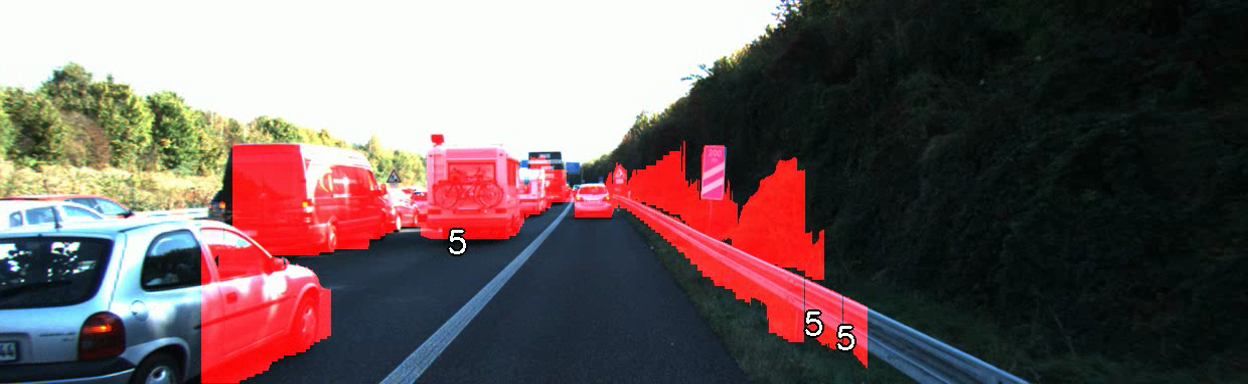
\includegraphics[width=\textwidth]{basic_vdisparity_good.png}
     \caption{Пример удачной работы алгоритма выделения областей, отличных от поверхности земли }
     \label{fig:basic_vdisparity_good}
\end{figure}
\begin{figure}[]
     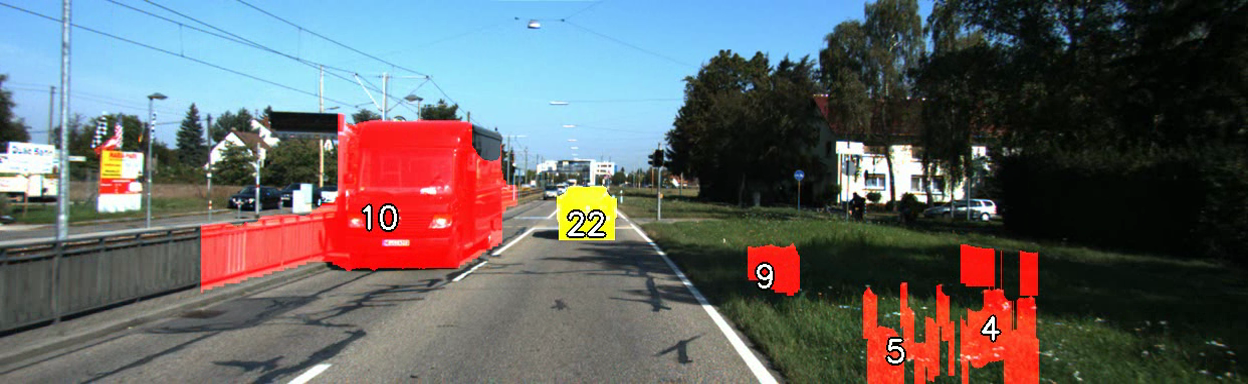
\includegraphics[width=\textwidth]{basic_vdisparity.png}
     \caption{Пример неудачной работы алгоритма выделения областей, отличных от поверхности земли }
     \label{fig:basic_vdisparity}
\end{figure}
\begin{figure}[]
     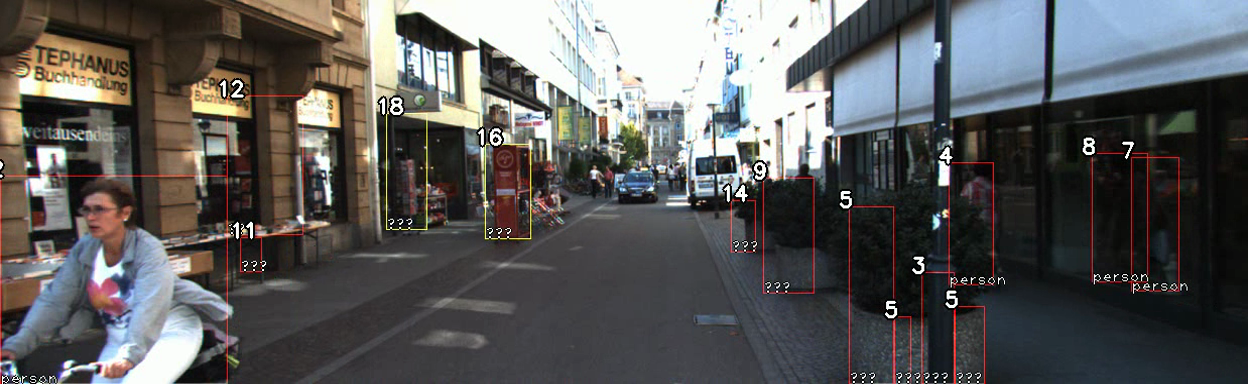
\includegraphics[width=\textwidth]{stixel_boxes.png}
     \caption{Пример сегментации области, содержащей препятствия, на отдельные объекты }
     \label{fig:stixel_boxes}
\end{figure}
\begin{figure}[]
     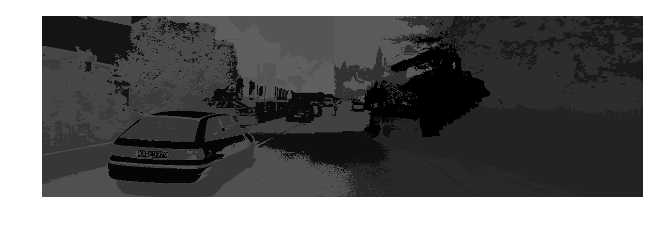
\includegraphics[width=\textwidth]{download.png}
     \caption{Выделение объектов алгоритмом из статьи \cite{franke20056d}. Разные интенсивности соответствуют разным объектам}
     \label{fig:6d}
\end{figure}
\begin{figure}[]
     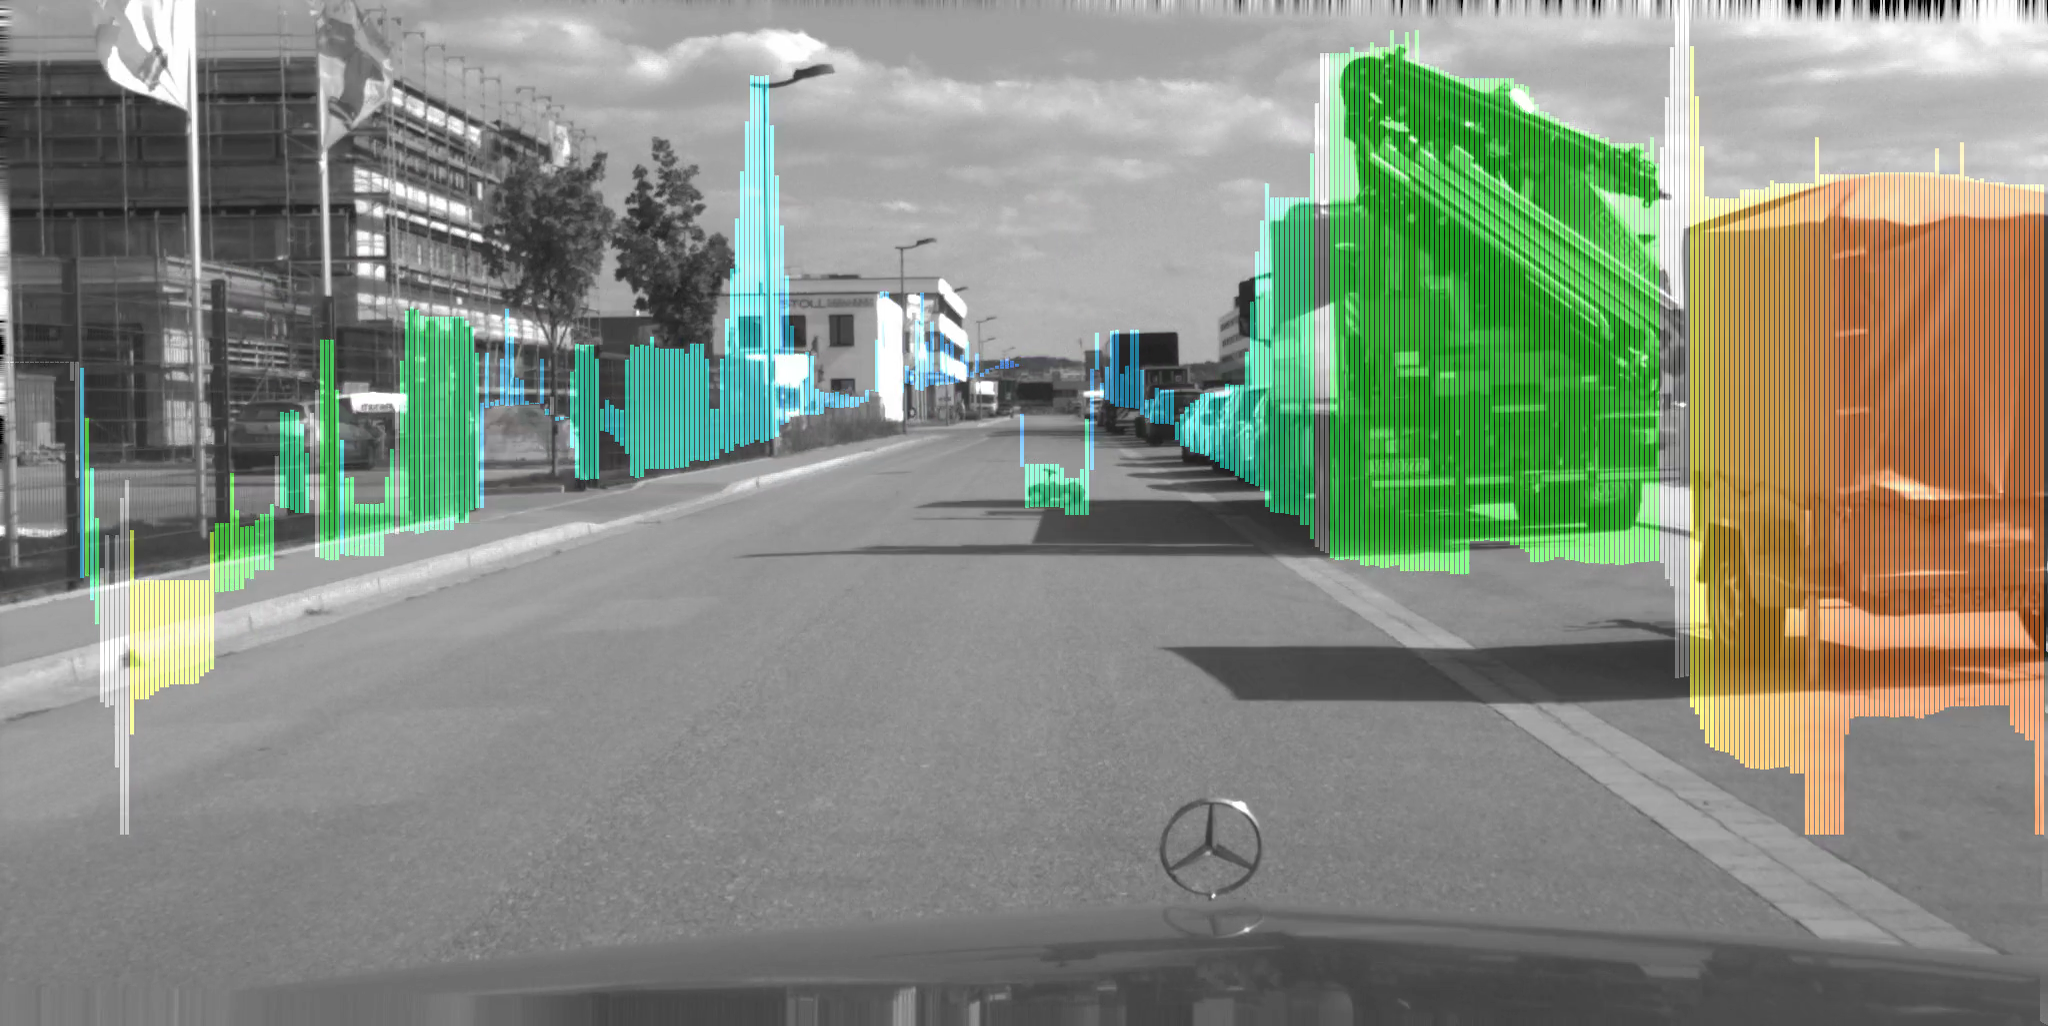
\includegraphics[width=\textwidth]{small_object.png}
     \caption{Выделение небольших объектов с помощью стикселей }
     \label{fig:small}
\end{figure}
\begin{figure}[]
     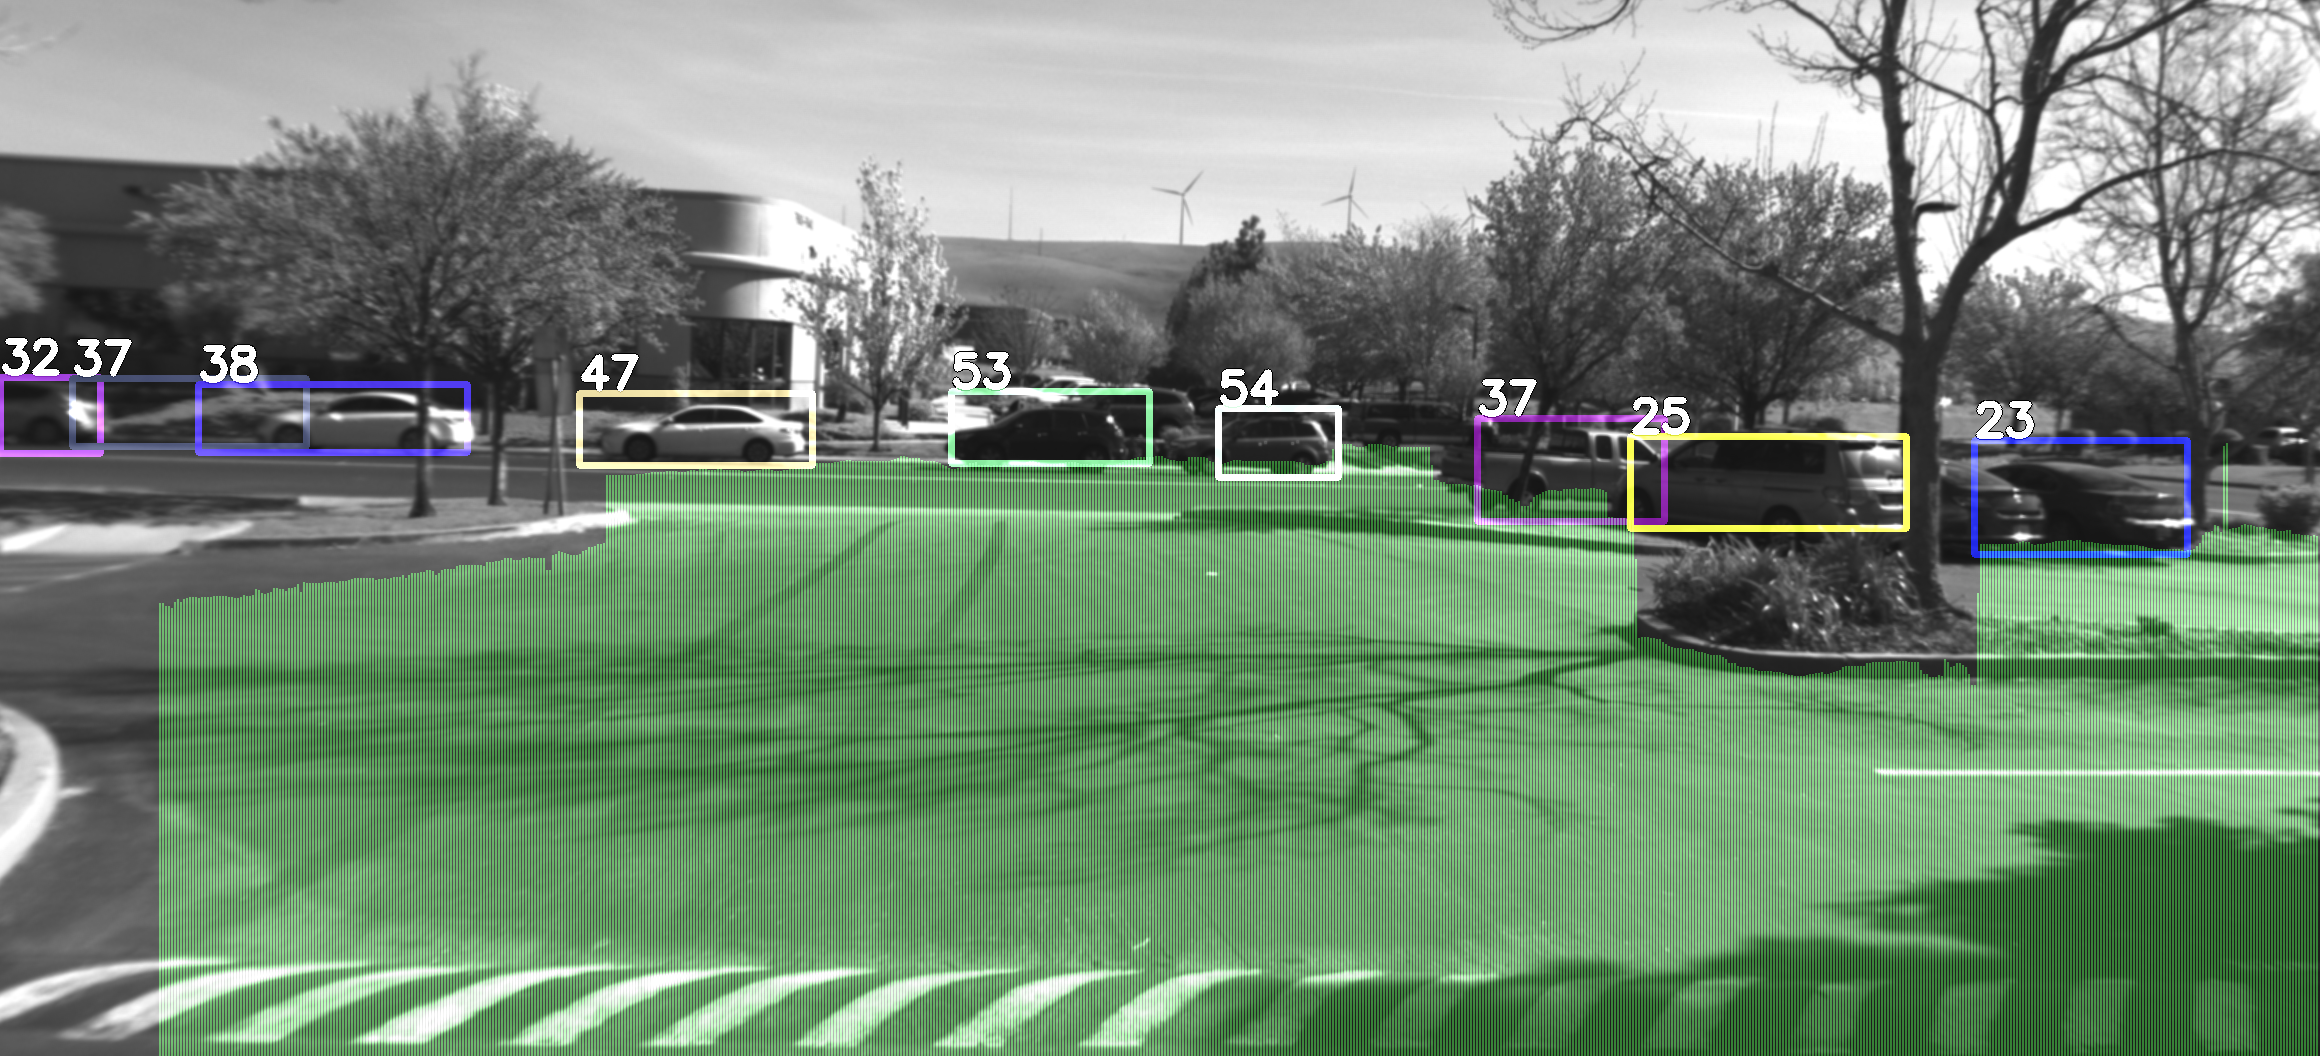
\includegraphics[width=\textwidth]{onroad.png}
     \caption{Пример работы стикселей, зелёным выделено безопасное пространство }
     \label{fig:stix_onroad}
\end{figure}
\begin{figure}[]
     \includegraphics[width=\textwidth]{offroad.png}
     \caption{Пример работы стикселей, зелёным выделено безопасное пространство }
     \label{fig:stix_offroad}
\end{figure}
\begin{figure}[]
     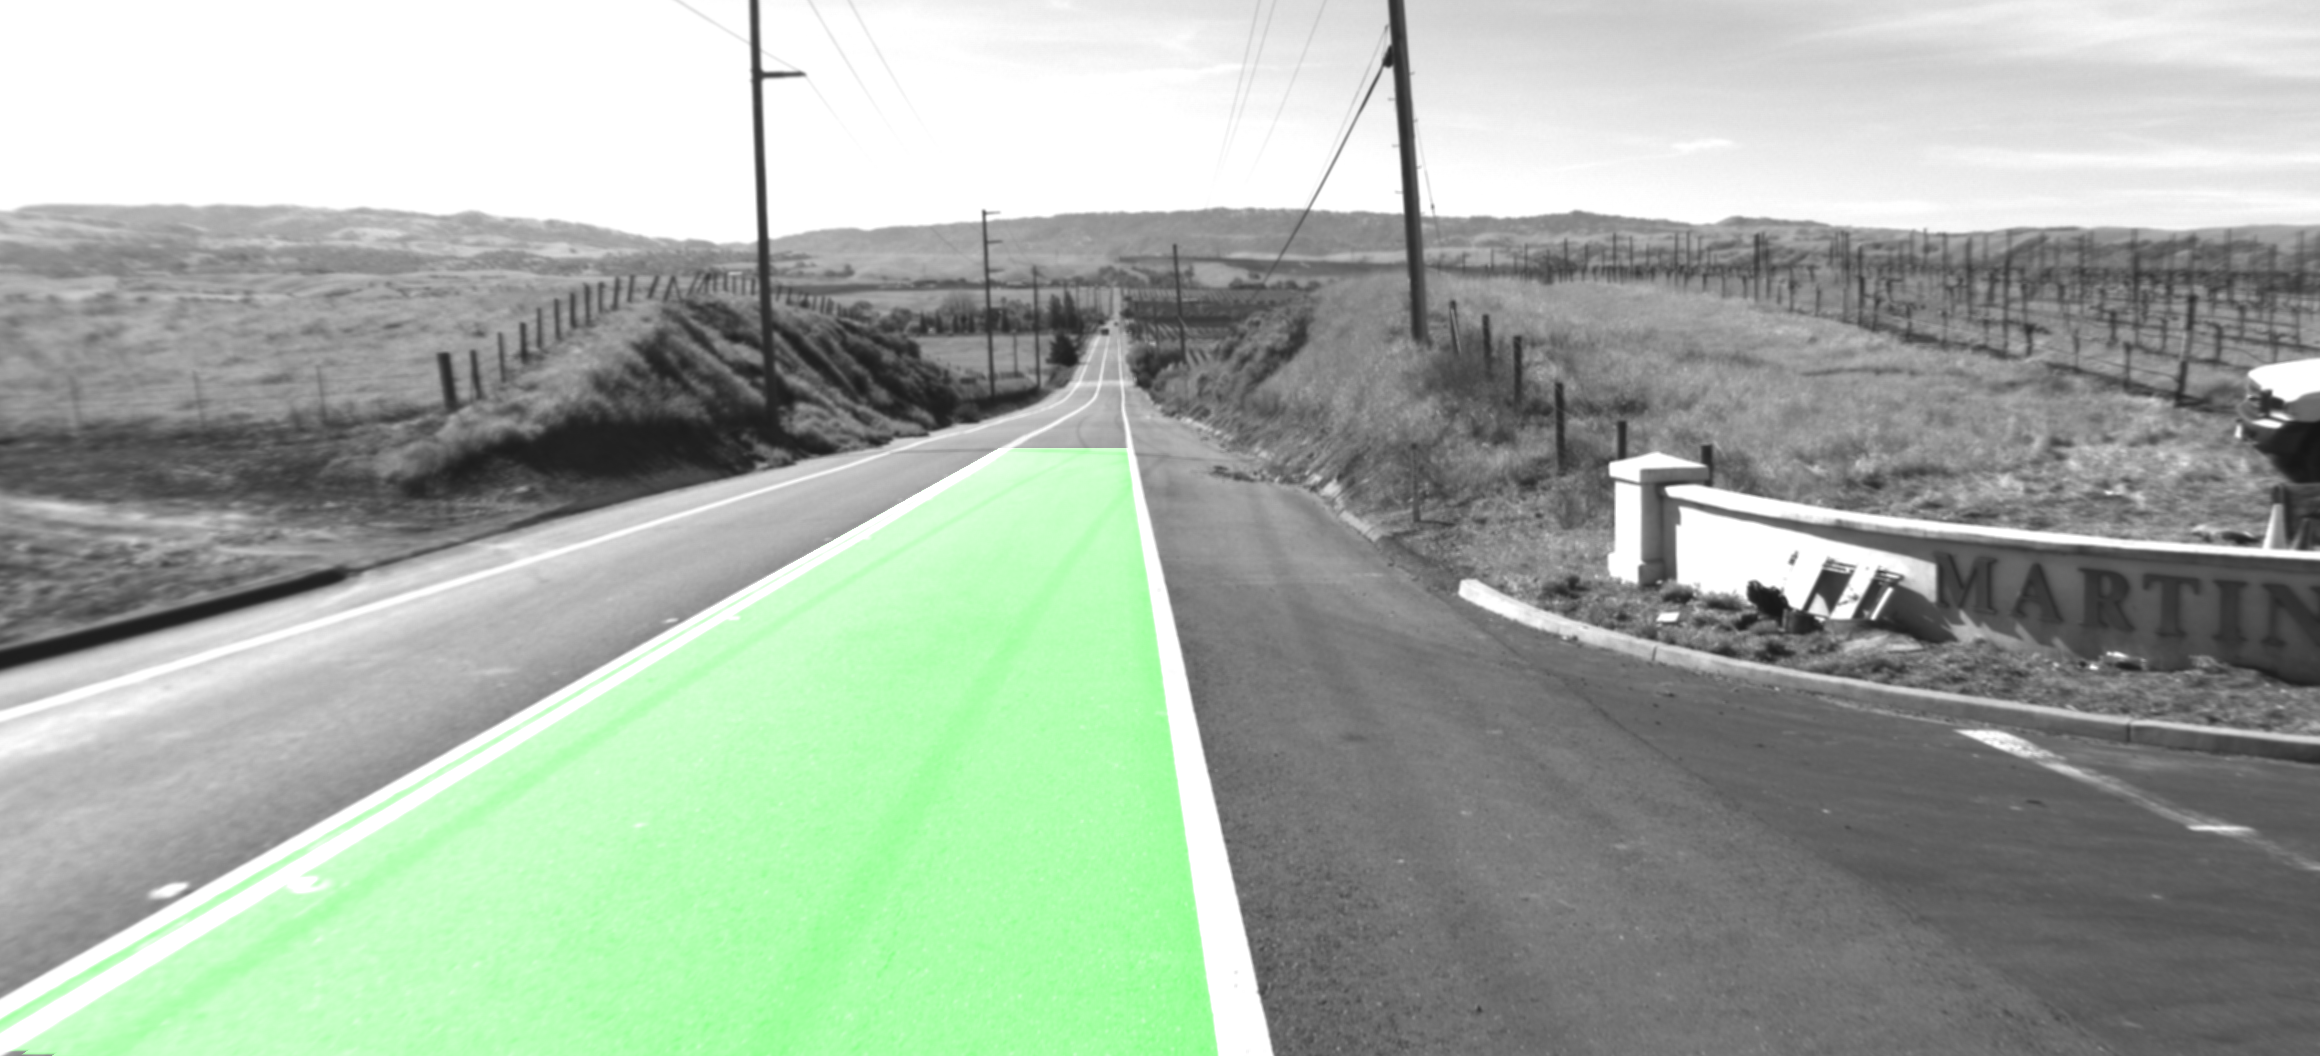
\includegraphics[width=\textwidth]{324.png}
     \caption{Пример работы алгоритма выделения дорожных маркеров с помощью цвета }
     \label{fig:color_markers}
\end{figure}
\begin{figure}[]
     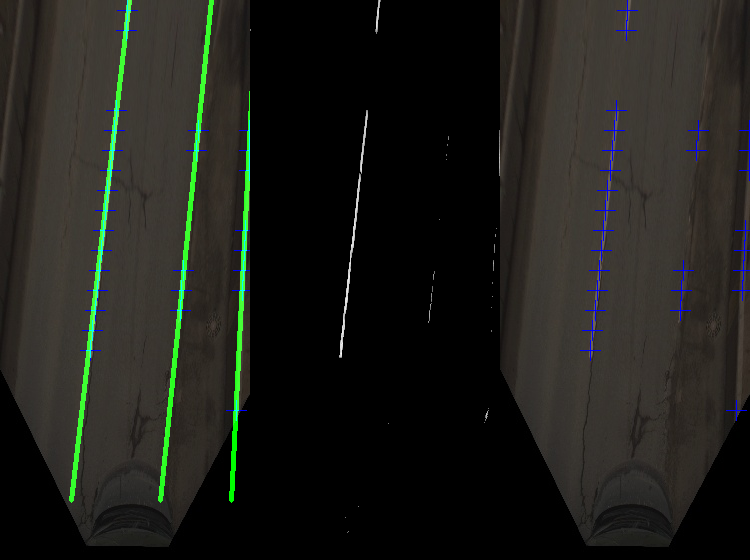
\includegraphics[width=\textwidth]{0000000026.png}
     \caption{Пример работы алгоритма выделения дорожных маркеров с помощью алгоритма RANSAC }
     \label{fig:ransac_markers}
\end{figure}
\newpage

\bibliographystyle{ugost2008ls}
\bibliography{diploma.bib}
\end{document}


